\documentclass[12pt]{article}
\usepackage[english]{babel}
\usepackage{natbib}
\usepackage{url}
\usepackage[utf8x]{inputenc}
\usepackage{amsmath}
\usepackage{graphicx}
\graphicspath{{images/}}
\usepackage{parskip}
\usepackage{fancyhdr}
\usepackage{vmargin}
\usepackage{subfig}
\usepackage{float}
\setmarginsrb{3 cm}{2.5 cm}{3 cm}{2.5 cm}{1 cm}{1.5 cm}{1 cm}{1.5 cm}

\title{3 - Class AB Output Stage (Prelab)}                             % Title
\author{John Wu \\ Ian Smith \\ Bilal Yousuf}                               % Author
\date{\today}                                                           % Date

\makeatletter
\let\thetitle\@title
\let\theauthor\@author
\let\thedate\@date
\makeatother

\pagestyle{fancy}
\fancyhf{}
\rhead{\theauthor}
\lhead{\thetitle}
\cfoot{\thepage}

\begin{document}

%%%%%%%%%%%%%%%%%%%%%%%%%%%%%%%%%%%%%%%%%%%%%%%%%%%%%%%%%%%%%%%%%%%%%%%%%%%%%%%%%%%%%%%%%

\begin{titlepage}
    \centering
    \vspace*{0.5 cm}
    
\includegraphics[scale = 0.07]{mcgill-logo.png}\\[1.0 cm]   % University Logo
    \textsc{\LARGE McGill University}\\[1.0 cm]   % University Name
    \textsc{\Large ECSE 335}\\[0.5 cm]               % Course Code
    \textsc{\large Microelectronic Labs}\\[0.5 cm]               % Course Name
    \rule{\linewidth}{0.2 mm} \\[0.4 cm]
    { \huge \bfseries \thetitle}\\
    \rule{\linewidth}{0.2 mm} \\[1.5 cm]
    \begin{minipage}{0.4\textwidth}
        \begin{flushleft} \large
            \emph{Authors (Group X):}\\
            \theauthor
            \end{flushleft}
            \end{minipage}~
            \begin{minipage}{0.4\textwidth}
            \begin{flushright} \large
            \emph{Student Number:} \\
            260612056 \\ 260612056 \\ 260680182                                  % Your Student Number
        \end{flushright}
    \end{minipage}\\[2 cm]
 
    {\large \thedate}\\[2 cm]
 
    \vfill
    
\end{titlepage}

%%%%%%%%%%%%%%%%%%%%%%%%%%%%%%%%%%%%%%%%%%%%%%%%%%%%%%%%%%%%%%%%%%%%%%%%%%%%%%%%%%%%%%%%%

\section*{3.1 Preparation}

\begin{figure}[H]
\centering
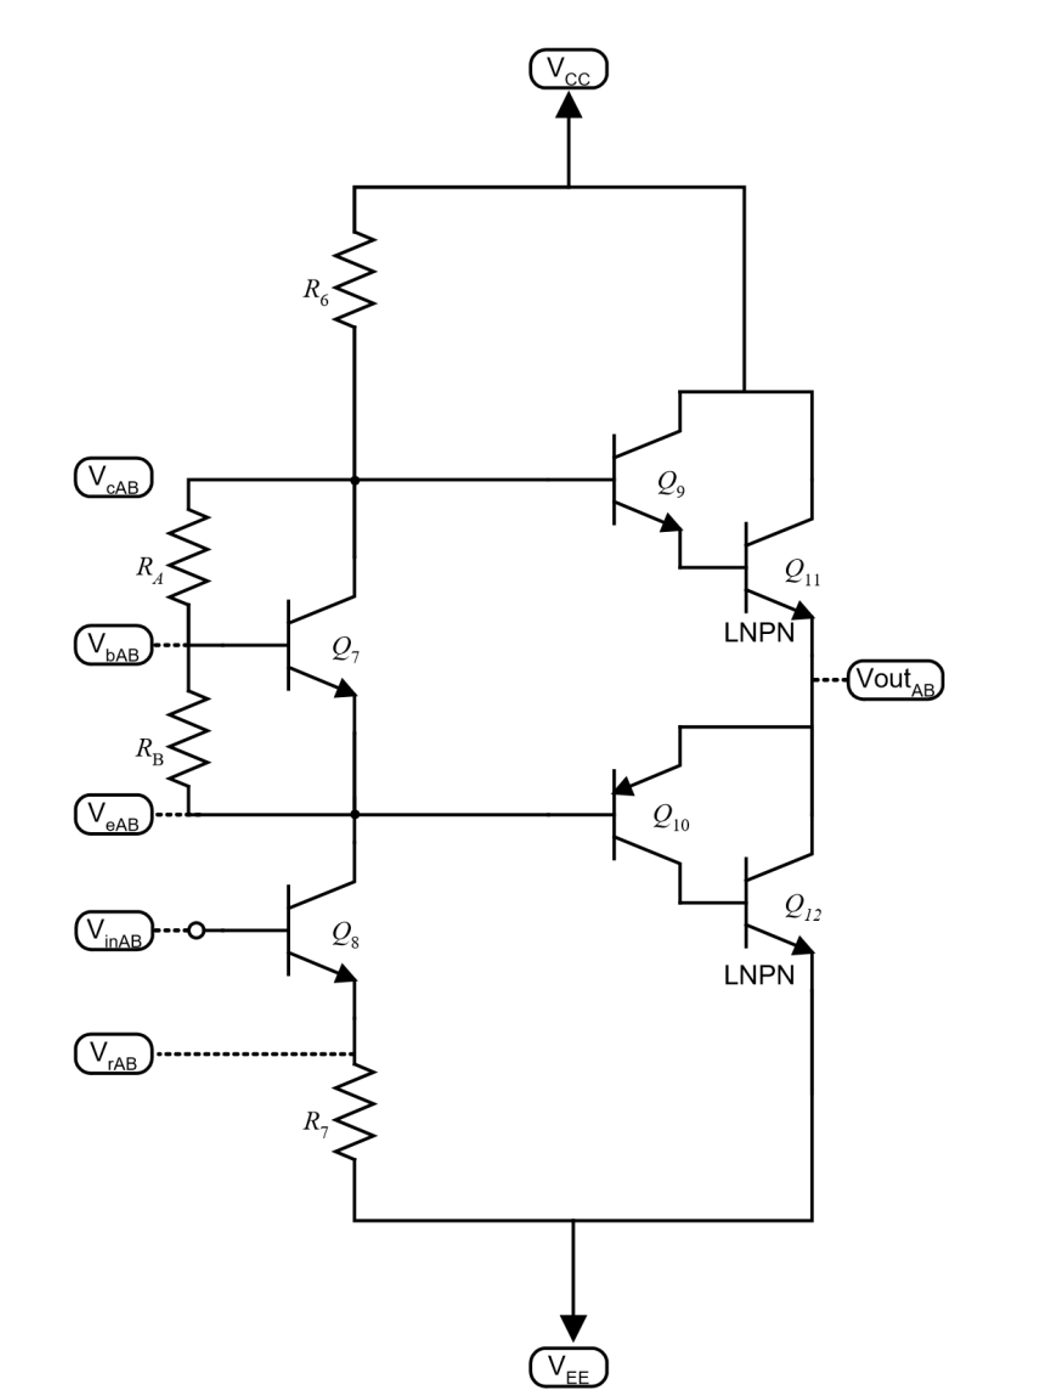
\includegraphics[width=0.8\textwidth]{main.PNG}
\caption{Class AB Output Stage - Full Circuit}
\end{figure}

\begin{figure}[H]
\centering
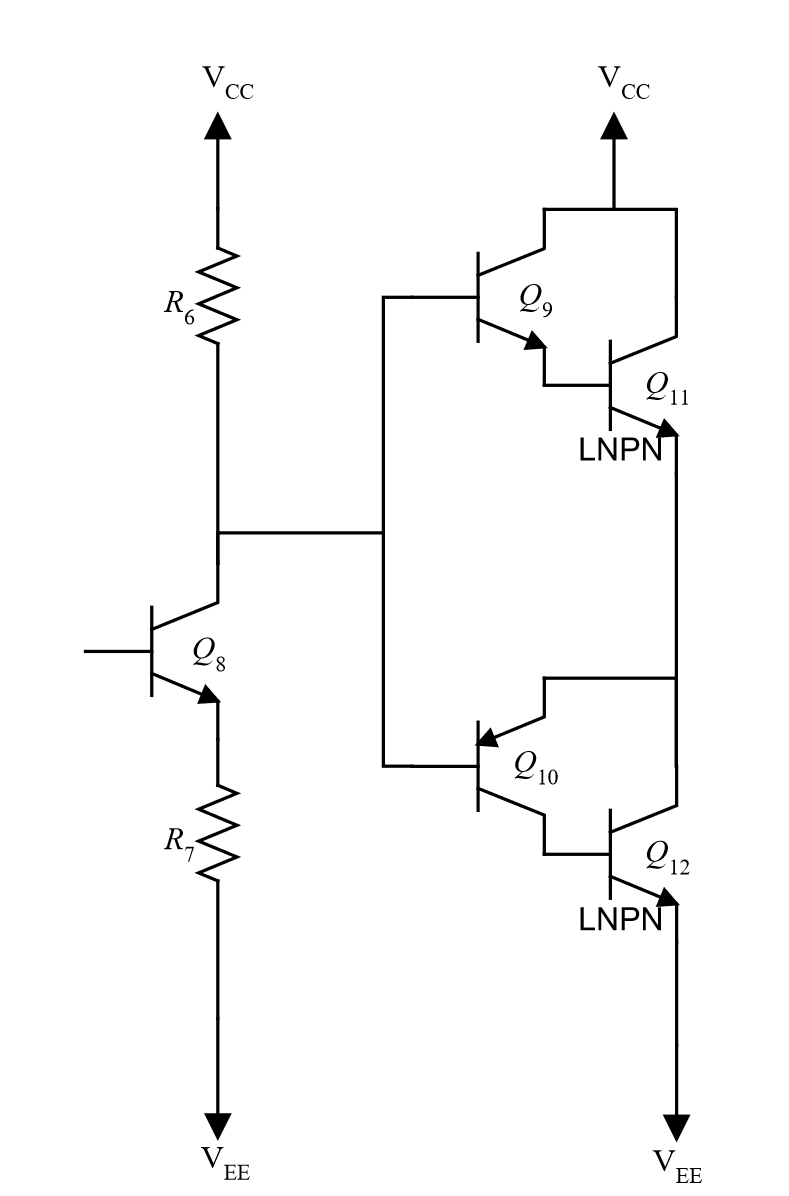
\includegraphics[width=0.4\textwidth]{shorted.PNG}
\caption{Modified Class B Output Stage - $V_{BE}$ multiplier shorted}
\end{figure}

\begin{figure}[H]
\centering
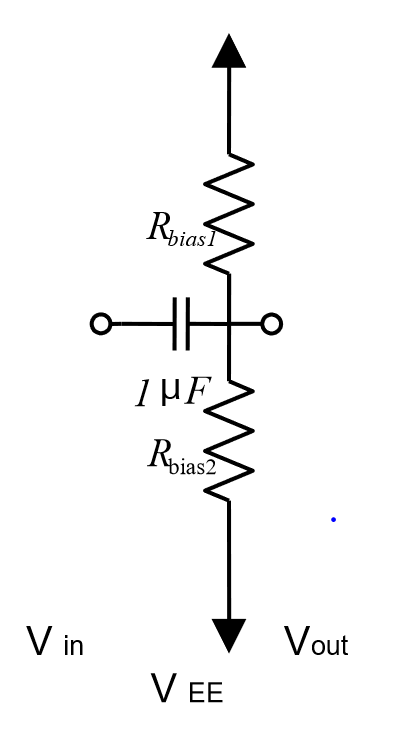
\includegraphics[width=0.3\textwidth]{bias.PNG}
\caption{Input biasing network used for standalone output stage testing}
\end{figure}

\subsection*{3.1.2 Considering this circuit will be used as an output stage in an operational amplifier, what are the main characteristics that it must have?}

Since the circuit will be used as an output stage in an operational amplifier, it must have the following characteristics in its most ideal form.


\begin{itemize}
    \item Infinite open-loop gain.
    \item Infinite bandwidth due to ideal gain.
    \item Infinite or zero common mode rejection ratio (CMRR).
    \item Infinite input impedance.
    \item Zero output impedance.
\end{itemize}

In general, these ideal characteristics will not be the actual case, but it will aim to be as close to these idealistic values as possible in order to deliver large currents to a small load - the goal of an op-amp.

\subsection*{3.2.3 Design the Class AB output stage circuit in Figure 3.1. Check that the following specifications are met: the quiescent current (zero input signal) is 0.5 mA, and that the output stage is capable of supplying 6 V p-p to a 330 $\Omega$ load without significant distortion, and the output stage provides a unloaded (disconnected load) gain of 10V/V. Remember that when the circuit is tested alone, the biasing stage in Figure 3.3 needs to be used. }

Requirements: $I_{quiescent} = 0.5mA$ and $A_{unloaded} = 10V/V$. \\

Choose $V_{cAB} - 1.5V$ to ensure enough voltage for biasing the transistors on. \\

$V_{cc} - I_{quiescent} R_6 = V_{cAB} \rightarrow 5 - 0.5 mA (R_6) = 1.5 \Rightarrow R_6 = 7000 \Omega$

$R_B = V_{be7} / I_{quiescent} \rightarrow R_B = 0.7 / 0.5 mA \Rightarrow R_B = 1400 \Omega $ \\ 

Choose $V_{BB}$ to be 2V, similarly.\\

$V_{BB} = I (R_A + R_B) \rightarrow 2 V = 0.5mA (R_A + 14000 \Omega) \Rightarrow R_A = 2600 \Omega$ \\

Designing for no load gain of 10 V/V. \\

$r_{o7} = V_A / I_C \rightarrow r_{o7} = 74 V / 0.125 mA \Rightarrow r_{o7} = 592.24K \Omega$ \\

$A_{unloaded} = [ r_{o7} || (R_A + R_B) + R_6 ] / R_7 $ \\

$\rightarrow 10 V/V = [ 592 K || (2600 + 1400) + 7000 ] / R_7$ \\

$\Rightarrow R_7 = 1K \Omega$ (Approximately) \\

Find resistor values for biasing circuit \\

$V_{in-AB} = -V_{EE} + 0.5(R_7) = -4.46 V$ 

$4.46 = 10 [ R_{bias2} / (R_{bias1} + R_{bias2}) ] \rightarrow 0.8 R_{bias1} = R_{bias2}$ \\

$\Rightarrow$ Choose $R_{bias1} = 1K \Omega$ and $R_{bias2} = 800 \Omega$

\subsection*{3.1.4 Determine the input resistance. Comment on how it is different to a small-signal amplifier.}


$R_{in} = (\beta + 1)(R_E+ R_e) = 101(1000+50) = 106K \Omega$

The difference from the small-signal amplifier in the previous lab is is the factor of 2 in the expression of $R_{in}$ for a small signal amplifier when measured as a differential.

\subsection*{3.1.5 Plot the frequency response and comment. Remember to include 5pF parasitic capacitors to ground for each pin, and account for the parasitics of the oscilloscope.}

As shown in the plot, the midband gain is close to 0dB, confirming the desired close to unity gain behaviour. The upper 3dB cutoff frequency is within the order of magnitude of 1MHz


\subsection*{3.1.6 Plot the voltage transfer characteristic, and then perform a transient analysis of both designed circuits. Document the maximal output range.}

From the graph above, we can observe a voltage swing from approximately -3.2 to 4.7 which centers at the input of 0.5V


\subsection*{3.1.7 In summary, what are the advantages and limitations of the class AB output stage?}

The advantage is that is solves the problem of the "dead-zone" which exists in the transfer characteristic of the class B output stage. \\

The limitations are the power inefficiencies which exist with the circuit as the transistors are all ways biased on. 

\subsection*{3.1.8 What is the purpose of transistor $Q_{12}$?}

The purpose of the the transistor is so that it can be combined with transistor $Q_11$ to form a darlington pair configuration which allows larger currents to be delivered to the load despite having a small base current.

\subsection*{3.1.9 What are the advantages and disadvantages of having an internal gain to the Class AB output stage, compared to having the bulk of the gain provided only by the differential pair?   }




\end{document}